\chapter{Machine Learning}
\label{sec:ml}
The scientific field of \acrfull{ml} if often seen as a part of the greater field of \acrfull{ai}\cite[3]{Alpaydin10}, and the term was coined by Arthur Samuel in \citeyear{samuelmachinelearning} \cite{samuelmachinelearning}. An \acrshort{ml} algorithm builds a model based on a dataset, with the goal of making predictions or classifications without being explicitly programmed how to do so. 

Some problems can easily be solved by programming an explicit algorithm (e.g. sorting a list, or \acrshort{fbp} reconstruction), however there are many cases where an exact algorithm simply does not exist (e.g. telling spam emails from legitimate emails) \cite[1]{Alpaydin10}. Often we have access to a large amount of sample data (e.g. emails where some have been manually flagged as spam) pertaining to the issue, however what is lacking is a suitable algorithm to parse and classify all the data. This is where \acrshort{ml} comes in: an \acrshort{ml} model can be trained to discern differences in a dataset without being explicitly told what to look for. So long as there is a sufficient amount of data to train the model with, it may be able to find a pattern in the data and thereby augment or enhance the data, or predict or classify new data \cite[2-4]{Alpaydin10}. 

There are many different \acrshort{ml} algorithms, however in this thesis only the class of neural networks will be discussed and the focus will be on supervised learning. 
\todo[inline]{This chapter contains ...}

\section{Components of a Neural Network}
\label{sec:ml:componentsofaneuralnetwork}
Neural networks were initially designed to simulate the human brain and how it learns and adapts to new information \cite{McCulloch1943}. Because of this, the basic building block of a neural network is called a neuron. Several neurons builds up a layer, and several layers build up a neural network. Neurons in different layers have connections to each other (i.e. neurons in layer 1 are connected to neurons in layer 2), and these connections have weights and biases. A simple schematic of this can be seen in \cref{fig:neuralnetwork}. The value of a neuron is a real number, and can be given as \cite[81]{Wang2003}
\begin{equation}
    \label{eq:neuron}
    Y_{k} = \sigma\left(\sum_{j=0}^{m}w_{kj}x_j + \lambda \right),
\end{equation}
where $k$ refers to which neuron it is, $m$ is the number of inputs to the neuron, $w_{kj}$ is the weight of connection $j$, $x_j$ is the output value of neuron $j$ into neuron $k$, $\lambda$ is a bias term, and $\sigma$ is the activation (or transfer) function, which will be introduced later. It is thus a weighted sum of the values of the neurons in the previous layer (or more precisely, of all the input neurons to a given neuron, which often is the previous layer). Note that this describes a simple fully connected feedforward \acrfull{ann}, and other types of neural networks may contain other types of layers \cite{oshea2015introduction}.

\begin{figure}[htbp]  
    \centering
    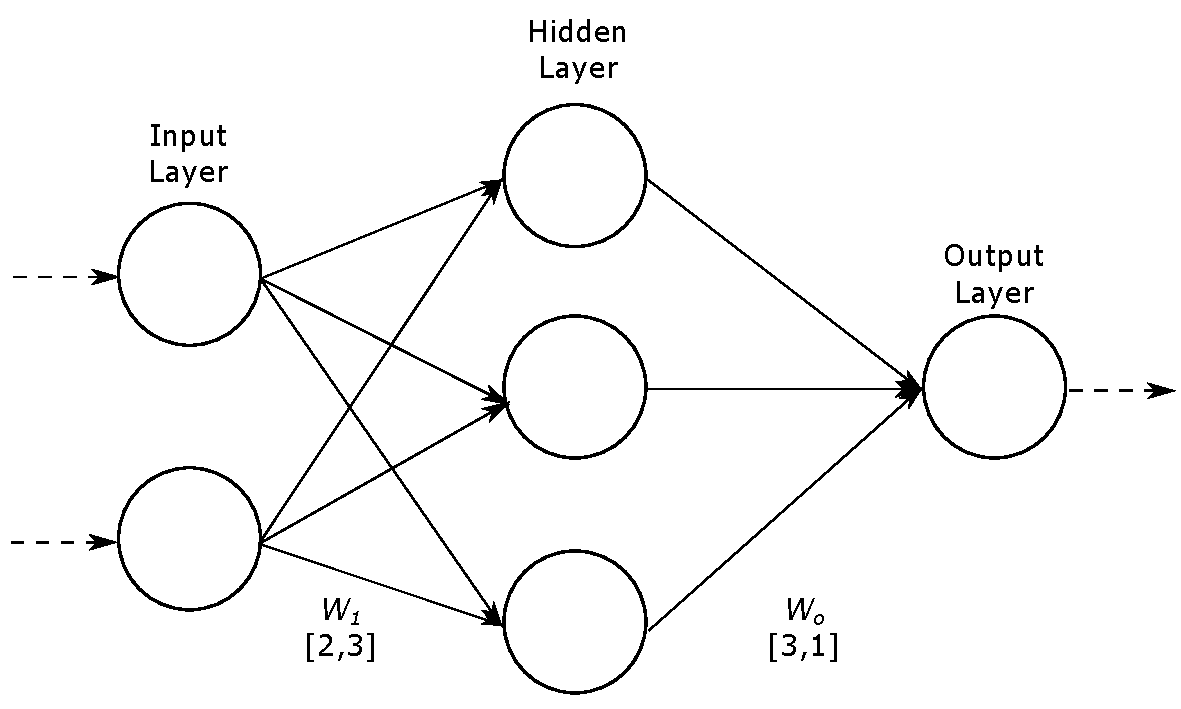
\includegraphics[width=.8\textwidth]{figures/neuralnetwork.pdf}
    \caption[Neural network example]{A simple schematic of a neural network. Each circle represents a neuron, the solid arrows represent connections between neurons, and the dotted arrows represent input and output channels. The dimensions of the network parameters are denoted as $W_n$, where $n$ refers to the layer the parameters input into. This network specifically is a fully connected feedforward \acrlong{ann} with one hidden layer. }
    \label{fig:neuralnetwork}
\end{figure}

The activation function, also known as the transfer function, is denoted as $\sigma$. Its purpose is to bound the value of a neuron so that the network is not crippled by divergent neurons \cite[81]{Wang2003}. There are many different activation functions, and some examples are presented in \cref{tab:activationfunctions} and plotted in \cref{fig:activationfunctions}. Furthermore, the activation function is used to introduce nonlinearity to the network\footnote{For this reason, the identity activation function $f(x)=x$ generally performs poorly.}, and it can be shown that a two-layer deep neural network with a nonlinear activation function is a universal function approximator \cite{Cybenko1989}. 

\begin{table}[htbp]
    \centering
    \caption[Activation functions]{Overview of some of the commonly used activation functions in neural networks. }
    \label{tab:activationfunctions}
    \begin{tabular}{ll}
    \hline
    Name & Function, $f(x)$ \\
    \hhline{==}
    Identity & $x$ \\
    Rectified Linear Unit (ReLU) & $\max\left(0, x\right)$ \\
    Leaky Rectified Linear Unit (LReLU) & $\max\left(\alpha x, x\right), \alpha\in[0,1]$ \\
    Logistic/soft step & $\frac{1}{1+e^{-x}}$  \\
    tanh & $\frac{e^x - e^{-x}}{e^x + e^{-x}}$ \\
    Softplus & $\ln\left(1+e^x\right)$ \\
    \hline
    \end{tabular}
\end{table}

\begin{figure}[htbp]  
    \centering
    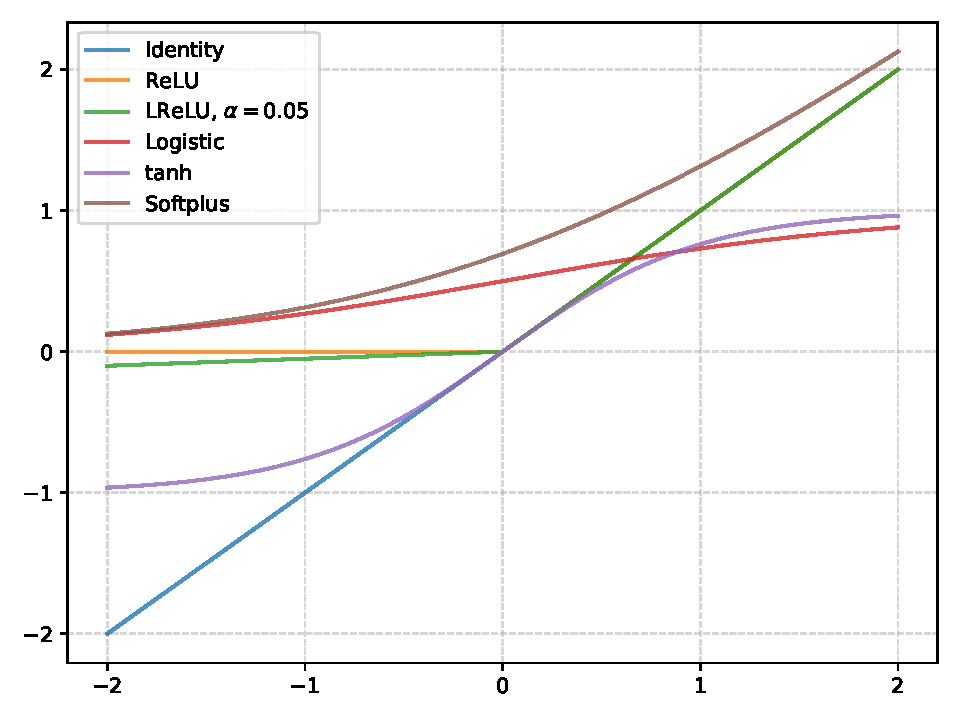
\includegraphics[width=.8\textwidth]{figures/activationfunctions.pdf}
    \caption[Activation functions]{Plot showing a selection of activation functions for $x\in[-2,2]$. Note that identity, ReLU, and LReLU are overlapping for $x\in[0,-2]$. }
    \label{fig:activationfunctions}
\end{figure}

The output of a neural network can be defined to be any shape. Depicted in \cref{fig:neuralnetwork} the output is a singular value, however it could just as well have been defined as a vector of values. If the output is a singular value it can for instance be interpreted as a probability, however if it is a vector of length $n$ it can be seen as $n$ probabilites of different events or features. The output of a neural network is often called a feature map, because it can be seen as a mapping of the features of the input data. 

As an example, if a neural network is trained with a dataset containing images of handwritten digits $0-9$, an output with a size of $10$ could contain probabilities of a given image containing a specific digit where each output value is the probability of one digit. One well-known dataset that is often used for this exact problem is the MNIST dataset \cite{mnist}.


\section{Neural Network Types}
There are many different types of neural networks that are suited for different problems. Here, a selection of types that lead up to the \acrfull{gan} structure used in this thesis will be introduced. 

\subsection{Convolutional Neural Network}
A \acrfull{cnn} builds upon the structure of the \acrshort{ann}, however it adds a new type of layer: the convolutional layer. Instead of containing a set of neurons, this layer contains one (or more) convolutional kernel(s), and performs a convolution of the input to the layer with the kernel(s). This type of network was first introduced in \citeyear{lecun1999object}\footnote{There is some disagreement around whether the paper by LeCun in \citeyear{lecun1999object} \cite{lecun1999object} was truly the introduction of \acrshort{cnn}s, however it is often seen as it. }, and has shown to work very well for many different image related tasks \cite{lecun1999object,alexnet}. Because of the nature of the convolutions, it allows the network to utilize 2D information by performing 2D convolutions\footnote{Likewise higher-dimensional information may be used by performing higher-dimensional convolutions \cite{8353466}. }. This has been shown to perform exceptionally well in image processing tasks \cite{alexnet,oshea2015introduction}. 

The convolution operator is defined as 
\begin{equation}
    \label{eq:convolution}
    g(x,y) = \omega \ast f(x,y) = \sum_{dx=-a}^{a}\sum_{dy=-b}^{b} \omega(dx,dy)f(x+dx,y+dy),
\end{equation}
where $g(x,y)$ is the convoluted matrix, $f(x,y)$ is the original matrix, and $\omega$ is a convolution kernel of dimension $(2a+1,2b+1)$\footnote{The dimensions of the kernel are typically square and odd, such as $3\times3$ or $5\times5$, giving $dx,dy\in[-1,1]$ or $dx,dy\in[-2,2]$. }. For simplicity, kernel dimensions will be refered to as $a\times b$ where $a$ and $b$ simply represent the kernel dimensions, and not the half-dimension as would correspond to \cref{eq:convolution}. 

A visualization of what the convolution of a matrix (which could represent an image) with a given kernel can be seen in \cref{fig:convolution}. Here, the kernel dimensions are $3\times3$. The output matrix has reduced dimensions corresponding to the kernel dimensions. The reduction can be given as 
\begin{equation}
    \left( x_o,y_o \right) = \left( x_i - \left(a - 1\right), x_i - \left( b - 1 \right) \right),
\end{equation}
where $(x_o,y_o)$ are the output dimensions, $(x_i,y_i)$ are the input dimensions, and $a$ and $b$ are the kernel dimensions. In some situations it may not be wanted to reduce the dimensions of the input, and padding the input with zeroes on all sides can be used to combat this. This technique is called zero-padding \cite{oshea2015introduction}. 
\begin{figure}[htbp]  
    \centering
    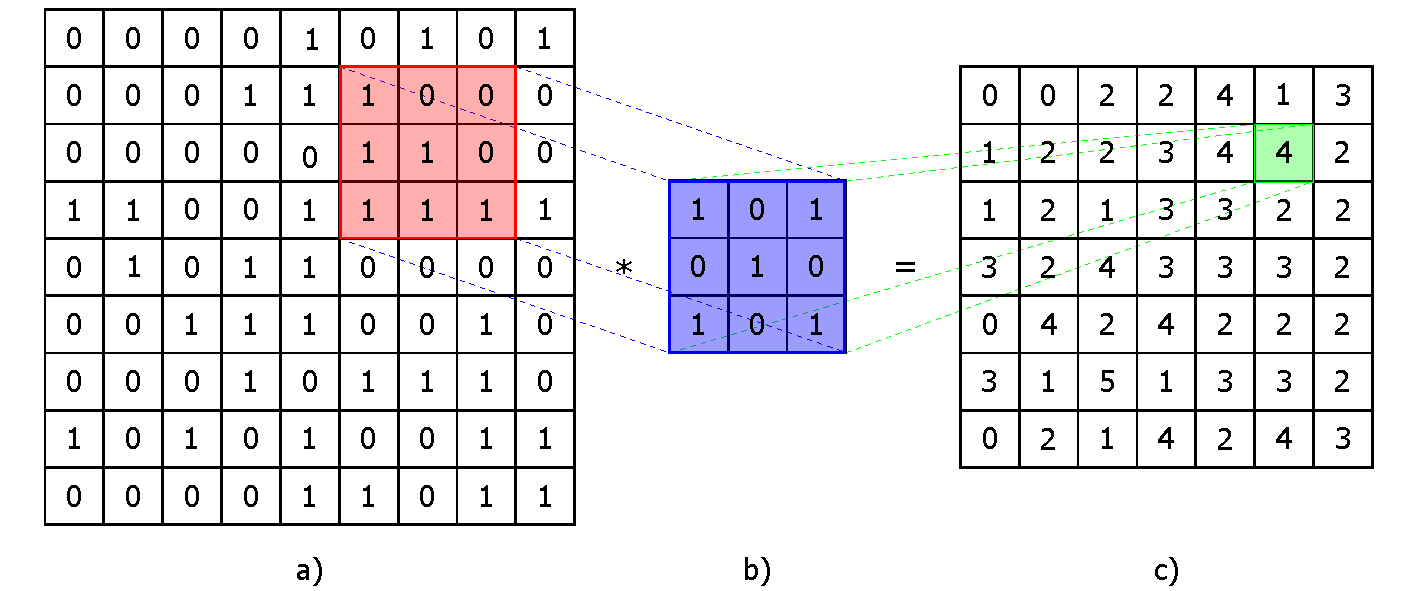
\includegraphics[width=.85\textwidth]{figures/convolution.pdf}
    \caption[Convolution example]{An example showing how a convolution works. This figure depicts: a) an input matrix of dimension $(9,9)$ (e.g. an image), b) a $3\times3$ convolutional kernel, and c) the resulting convolution of dimension $(7,7)$. This convolution also has a stride of 1. Note that the output dimension is smaller than the input dimension. }
    \label{fig:convolution}
\end{figure}

Multiple convolutional kernels can be used in parallel in each convolutional layer. The number of kernels is then refered to as the number of channels. 

The stride of a convolution is how far the kernel shifts \cite{oshea2015introduction}. In the example given in \cref{fig:convolution}, the stride is 1. If the stride were set to 2, the kernel would shift two units in the matrix for each output. This would mean less overlap between each value in the output, but also further reduction of the output dimensions. 

Often, pooling layers are included in \acrshort{cnn}s. These layers are used to down sample the feature maps after a convolutional layer by applying some pooling function (e.g. max, average, sum) to an area of the feature map, reducing the dimension. This can for instance be a $2\times2$ max pooling layer that looks at a $2\times2$ section of a feature map and replaces it with a single value corresponding to the maximum value of the original section. Pooling layers reduce the dimensions of the feature map corresponding to the size of the pooling (e.g. a $2\times2$ pooling layer reduces both dimensions of a feature map by a factor of $2$). 

The part of the convolution that a \acrshort{cnn} learns is the values in the convolutional kernel. Each layer of the \acrshort{cnn} may have several kernels that are applied in parallel (e.g. 32 kernels applied to the same input). Each kernel is often called a filter. One of the advantages of using convolution in neural networks is the reduction in the number of trainable parameters: a typical convolutional kernel contains $9-49$ parameters (for kernels of dimensions $3\times3$ to $7\times7$, however a fully connected feedforward network may have several thousands parameters for each layer\footnote{Consider an image of dimension $100\times100$. In a fully connected \acrshort{ann} there would have to be $100 \cdot 100 = 10^4$ connections from each neuron in one layer to the next layer for a total of $10^{8}$ connections, where each connection has a trainable parameter. In comparison, if using a \acrshort{cnn} with 32 channels (or kernels) of dimension $3\times3$ there are only a total of $32 \cdot 3 \cdot 3 = 288$ trainable parameters. }. 
\todo[inline]{Write about overfitting? Reduce number of trainable parameters helps avoid overfitting. }

\subsection{Encoder-Decoder Network}
\label{sec:ml:types:encoderdecoder}
An encoder-decoder network is a type of \acrshort{ann} that learns to copy its input to its output \cite{https://doi.org/10.1002/aic.690370209}. It consists of two parts (as the name suggests): an encoder, and a decoder. The task of the encoder is to take the input and encode it into a feature map. The decoder then takes the resulting feature map and decodes it into an output similar to the original input. A schematic of this structure can be seen in \cref{fig:encoderdecoder}. The encoder's goal is to extract the relevant information from the input, ignoring any signal noise or unwanted data. The decoder then recreates something similar to the original data from the "denoised" feature map. It is common to use \acrshort{cnn}s as both encoder and decoder, where consecutive layers in the encoder reduce the dimensions of the feature maps and consecutive layers in the decoder increase the dimensions of the feature maps. Encoder-decoder networks have been shown to perform well in many different tasks, such as image segmentation \cite{7803544} and PET image reconstruction \cite{HAGGSTROM2019253}.  

\begin{figure}[htbp]  
    \centering
    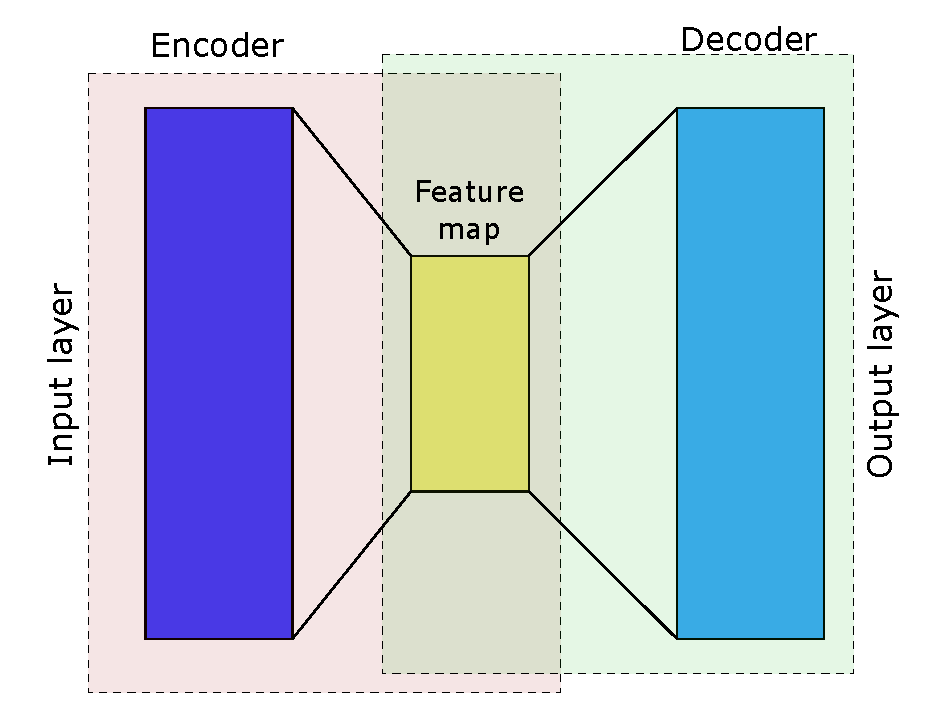
\includegraphics[width=.7\textwidth]{figures/encoderdecoder.pdf}
    \caption[Encoder-decoder network]{A simple schematic of the overall structure of an encoder-decoder network. It consists of two separable networks, the encoder and the decoder, working together. The input and output layers are of the same dimensions. }
    \label{fig:encoderdecoder}
\end{figure}

In an encoder-decoder network, the encoder and decoder are two separate networks that can work independently of each other. Another similar network structure that builds upon the encoder-decoder is the U-net convolutional network, originally proposed for biomedical image segmentation \cite{unet}. It also contains an encoder and a decoder part, however the two networks are not separable as there are skip-connections between layers in the encoder and layers in the decoder. In a normal encoder-decoder network there is first one mapping from the input $X$ to the feature map $L$, $X \mapsto L$, and then a mapping from the feature map $L$ to the output $Y$, $L \mapsto Y$. These two mappings are not dependent on each other. In the U-net architecture however,  the mapping in the decoder also depends on the input $X$, making it $[X+L] \mapsto Y$. 


\subsection{Generative Adversarial Network}
\label{sec:ml:types:gan}
\acrfull{gan}s were introduced in \citeyear{goodfellow2014gan} by Goodfellow et al.  as a novel method of estimating generating models via an adversarial process \cite{goodfellow2014gan}. This type of neural network consists of two separate networks: a generator and a discriminator. The generator, called $G$, captures the distribution of the training data and generates new samples from that distribution, while the discriminator $D$ estimates the probability that a given sample came from the training data (i.e. real sample) rather than being a generated sample from $G$. 

The two networks play a game, in the sense of game theory, where they try to minimize their own cost, or error rates, while at the same time maximizing the other network's cost \cite{goodfellow2020gan}. \acrshort{gan}s are designed to reach a Nash equilibrium at which neither of the two networks can reduce its costs without changing the other network's parameters \cite{liu2020tomogan}. As opposed to normal neural networks that are based on optimization to reduce their error rates, \acrshort{gan}s are based on game theory \cite{goodfellow2020gan}. 

To generate random samples from the distribution of the training data, a fully trained \acrshort{gan} is given random noise as input and then maps that to a random sample, such as in \cite{zhangsagan}. This allows the network to generate new samples that are similar, but not equal, to the training data. Another common use case for \acrshort{gan}s is to instead of feeding the network random noise as input, feeding it some data that needs augmentation. This has been used to denoise images and for image super-resolution \cite{8710893,Ledig_2017_CVPR}. 


\section{Training a Neural Network}
The process of tuning all the parameters (i.e. weights and biases) of a neural network is called training. During training, input data from a training dataset is forwards propagated through the network, and the resulting feature map is compared to an expected feature map (e.g. manually labeled data)\footnote{This is what is called supervised learning, as opposed to unsupervised learning where there is no ground truth answer to compare to, instead trying to learn some inherent structure of the data without explicit labels (e.g. clustering). }. The difference in these feature maps is calcuated using some loss function, and the loss is then backwards propagated through the network to update each and every parameter to reduce the loss. 

Generally, the entire training dataset is repeatedly passed through the network multiple times. Each full runthrough of the training dataset is called an epoch of training. This however can often introduce a problem: the training dataset can typically not fully fit in the computer memory at once. Therefore it is divided into mini batches, and after each mini batch the weights are adjusted. The propagation of one mini batch is often called one iteration, and thus one epoch consists of several iterations. The size of a mini batch is a tunable parameter, however typically it is in the range of $32-512$ (e.g. 128 in the well-known article by A. Krizhevsky et al. \cite{alexnet})\footnote{There is ongoing research into techniques to increase the batch size by several orders of magnitude as larger batches allow for easier parallelization, however large batch sizes have been shown to cause instability during training \cite{you2017large}. }. The size of a mini batch can sometimes also be refered to as the batch size. 

\subsection{Hyperparameters}
During training, the parameters of the neural network are automatically changed, however there are some parameters that are set manually beforehand. These are called hyperparameters \cite{claesen2015hyperparameter}. Some typical hyperparameters are:
\begin{itemize}
    \item Number of layers (i.e. depth of network).
    \item Size (or dimensions) of layers.
    \item Learning rate.
    \item Number of iterations to train the network (i.e. number of epochs).
    \item Mini batch size.
\end{itemize}

The process of choosing these hyperparameters is not an exact science, and there is research being done into finding ways of automatically tuning hyperparameters to their ideal configurations, called auto-tuning \cite{autotuning}.

\subsection{Loss Functions}
\label{sec:ml:training:lossfunctions}
To properly quantify the error, or loss, of a neural network one needs to define some metric. These are called loss functions. Depending on the problem type diferent loss functions may perform better than others, however there are some standard loss functions often used. Some of these, as well as some specific ones used in this thesis, will be presented here. The losses are calculated on a per-pixel basis and summed unless otherwise stated. 

Perhaps the most commonly used loss function is the \acrfull{mse}. It is closely related to the L2-norm, and it can be defined as
\begin{equation}
    \label{eq:lossmse}
    L_{\text{MSE}} = \frac{1}{N} \sum_{i=1}^N(Y_i - \hat{Y}_i)^2,
\end{equation}
where $Y$ is the correct (labeled) value,  $\hat{Y}$ is the predicted value, and $N$ is the number of samples. This often performs well, however in cases such as image processing or image super resolution it has shown to cause blurring \cite{7797130}.

Another similar loss function is the \acrfull{mae}, which is closely related to the L1-norm. It can be defined as
\begin{equation}
    \label{eq:lossmae}
    L_{\text{MAE}} = \frac{1}{N} \sum_{i=1}^N |Y_i - \hat{Y}_i|,
\end{equation}
with $Y$ and $\hat{Y}_i$ being the same as previously defined. This loss function does not over-penalize larger errors, and therefore may have different convergence properties than \acrshort{mse} \cite{7797130}. It has been shown to perform better than \acrshort{mse} in some image processing cases \cite{7797130,10.1002/mp.13713}. 

\todo[inline]{Write something about general norms for loss functions? }
% These loss functions can be generalized from $L1$ and $L2$ norms to $Ln$ norms

A more recently introduced loss function is the log-cosh loss function, defined as \cite{chen2019log}
\begin{equation}
    \label{eq:losslogcosh}
    L_{\text{Log-cosh}} = \frac{1}{a} \sum_{i=1}^N \log ( \cosh ( a ( Y_i - \hat{Y}_i))),
\end{equation}
where $Y$ and $\hat{Y}$ are as previously defined, $\log$ is the logarithm, $\cosh$ is the hyperbolic cosine function, and $a$ is some positive hyperparameter $a \in \mathbb{R}^+$. It behaves similar to \acrshort{mse} around the origin, and similar to \acrshort{mae} at other points. It has been shown to perform well in image processing related tasks \cite{7797130}.
% MSE, MAE, LogCosh, VGG, Adversarial
\todo[inline]{Wasserstein distance (for WGAN?)}
All the aforementioned loss functions rely on pixel-wise losses. Another type of loss functions that has shown to perform well in image processing related tasks is the use of a feature space based loss \cite{vggloss}. Specifically, this loss is based on measuring the difference in the feature space of the inferrence of a pre-trained network. Here, the pre-trained VGG network is used to measure a visual loss \cite{simonyan2015deep}. This specific loss function is termed visual loss, or VGG loss, and is defined as \cite{vggloss,liu2020tomogan}
\begin{equation}
    \label{eq:lossvgg}
    L_{\text{VGG}} = \sum_{i=1}^{N} \sum_{j=1}^{W_f} \sum_{k=1}^{H_f} \left(V_{\theta_{\text{VGG}}} (Y_i)_{j,k} - V_{\theta_{\text{VGG}}} (\hat{Y}_i)_{j,k} \right)^2,
\end{equation}
where $Y$ and $\hat{Y}$ are as previously defined, $V_{\theta_{\text{VGG}}}(Y)$ is the VGG feature map representation of image $Y$, and $W_f$ and $H_f$ are the dimensions of the feature maps extracted by the pre-trained VGG network. The VGG network is trained with natural images, specifically the ImageNet dataset \cite{deng2009imagenet}, however it has been shown to work well as a feature extractor for \acrshort{ct} images \cite{8340157}. 

Specific to \acrshort{gan}s is the adversarial loss. It is a measure of how well the generator network is able to produce samples that the discriminator network is unable to distinguish from real samples. It can be written as \cite{liu2020tomogan}
\begin{equation}
    \label{eq:lossadv}
    L_{\text{Adv}} = -\frac{1}{N} \sum_{i=1}^{N} D\left(  \hat{Y}_i \right),
\end{equation}
where $\hat{Y}_i$ is the generated guess from the generator network, and $D$ is the discriminator network giving a binary classification $D\left(\hat{Y}_i \right) \in [0,1]$ depending on whether it believes the given image is a real or generated one. Minimizing this loss ensures that the generator network produces samples that have a similar feature map (when extracted by the discriminator network) to real samples, and this process is the basis of \acrshort{gan}s. 


\subsubsection{Weighted loss}
In practise it is common to use a weighted sum of different loss functions. 
An example containing \acrshort{mse}, log-cosh, and VGG loss can be given as
\begin{equation}
    \label{eq:weightedloss}
    L_{\text{Total}} = \lambda_{\text{MSE}}L_{\text{MSE}} + \lambda_{\text{Log-cosh}}L_{\text{Log-cosh}} + \lambda_{\text{VGG}}L_{\text{VGG}},
\end{equation}
where $\lambda_N$ is a hyperparameter controlling the weight of $L_N$. 

\subsection{Backpropagation}
\todo[inline]{}

\subsection{Optimizers}
\todo[inline]{}

\subsubsection{Stochastic Gradient Descent}
The simplest type of optimizer that is often used in training neural networks is the \acrfull{sgd}. It is an iterative method for optimizing an objective function that has suitable smoothness properties (e.g. differentiability) \cite{stochasticgradientdescent}. It looks at the error in the feature map of the training network (when compared to the labeled ground truth), and calculates an approximation of the gradient needed to update all the weights in the network to reduce the error. Because of the use of mini batches during training of neural networks, the \acrshort{sgd} method only looks at a randomly selected subset of the whole training data and it is therefore called a stochastic method. The learning rate of \acrshort{sgd} is the step size used when updating the weights based on the calculated gradient.

\subsubsection{ADAM}
A more sophisticated optimization algorithm was introduced in \citeyear{kingma2015adam}, and is called ADAM. It is an algorithm for first-order gradient-based optimization of stochastic objective functions, based on adaptive estimates of lower-order moments \cite{kingma2015adam}. It can be seen as an extension to \acrshort{sgd}. While \acrshort{sgd} has one single learning rate, ADAM has one learning rate for each different parameter based on estimates of first and second moments of the gradients. 